% Vorlage fuer Studien- und Diplomarbeiten am Lehrstuhl fuer Betriebssysteme
% basiert auf scrbook, Doku dazu im scrguide.pdf (texdoc scrguide  oder google)

\documentclass[12pt,             % Schriftgroesse
               a4paper,          % Papierformat
               %liststotoc,      % (alt) Tabellen- und Abbildungsverzeichnis im Inhaltsverz.
               listof=totoc,     % Tabellen- und Abbildungsverzeichnis im Inhaltsverz.
               %idxtotoc,        % (alt) Index im Inhaltsverz. auffuehren
               index=totoc,      % Index im Inhaltsverz. auffuehren
               %bibtotoc,        % (alt) Literaturverzeichnis im Inhaltsverz. auffuehren
               bibliography=totoc,% Literaturverzeichnis im Inhaltsverz. auffuehren
               oneside,         % auskommentieren, wenn beidseitig gedruckt wird
                                 % default ist 'twoside'
               BCOR1cm,          % zusaetzlicher Bindungsrand
               %english,ngerman   % TODO : Englisch als weitere Sprache, Deutsch als Hauptsprache
               ngerman,english  % TODO : alternativ Deutsch als weitere und Englisch als Hauptsprache
               ]{scrbook}

%%%%%%%%%%%%%%%%%%%%%%%%%%%%%%%%%%%%%%%%%%%%%%%%%%%%%
% Pakete einbinden (Reihenfolge ist z.T. wichtig!)
%%%%%%%%%%%%%%%%%%%%%%%%%%%%%%%%%%%%%%%%%%%%%%%%%%%%%
\usepackage[latin1]{inputenc}   % Eingabezeichenkodierung, alternativ "ansinew"
                                % (Windows only) oder "utf8" fuer Unicode
\usepackage{cmap}               % Fuer schoene Ligaturen in PDFs
\usepackage[T1]{fontenc}        % u.a. Umlaute als ein Zeichen in der PDF-Datei
\usepackage{lmodern}            % Linux Modern Schriften auswaehlen
\usepackage{graphicx}           % Um Bilder einzubinden (mit \includegraphics)
\usepackage{makeidx}            % Falls ein Index erstellt werden soll, muessen
\usepackage{subfigure}
\usepackage{listings}
\makeindex                      %  die beiden Zeilen aktiviert werden.
                                %  zusaetzlich noch \printindex unten
\usepackage{units}              % Einheiten setzen mit z.B. \unit[10]{MB} und \unitfrac[100]{Mbit}{s}
%\usepackage{siunitx}           % Wesentlich umfangreicheres Einheiten Paket als Ersatz fuer "units"

% In dieser Datei koennen eigene Erweiterungen eingebracht werden
% HIER: Nur wenn noetig Datei my_includes.tex aendern
%% Hier eigene Definitionen und zus�tzlich gebrauchte Pakete einbinden
         % Eigene Pakete und Definitionen laden

% letztes:     ----------------------------------------------------------------------------------------------------
\usepackage{lfbsdasa}           % LfBS-Vorlage fuer Diplom- und Studienarbeiten 
                                %  mit Titelseite
% dieses sollte immer als letztes eingebunden werden, da es hyperref mitbringt 
% (welches wirklich das letzte ist)

%%%%%%%%%%%%%%%%%%%%%%%%%%%%%%%%%%%%%%%%%%%%%%%%%%%%%%%%%%%%%%%%%%%%%%%%%%%%%%%
% Hier beginnt das eigentliche Dokument
%%%%%%%%%%%%%%%%%%%%%%%%%%%%%%%%%%%%%%%%%%%%%%%%%%%%%%%%%%%%%%%%%%%%%%%%%%%%%%%
\begin{document}

%% Ein paar wichtige Details konfigurieren
%%----------------------------------------
% HIER: Details anpassen in my_config.tex
\author{Guillaume Qu�r�}                             % Name des Autors
\matnr{315804}                                       % Matrikel-Nummer
\reporttype{Projektarbeit}                          % Studienarbeit/Diplomarbeit/Bachelorarbeit/Masterarbeit
\titleEn{Introduction to userspace I/O control with embedded Linux on the BeagleBone}% Englischer Titel
\titleDe{Einf�hrung in die Userspace E/A-Steuerung mit Embedded Linux auf dem BeagleBone}
\addsupervisor{Dipl.-Ing. Georg Wassen}              % Betreuer

               % TODO : bearbeite Einstellungen in my_config.tex

%%%%%%%%%%%%%%%%%%%%%%%%%%%%%%%%%%%%%%%%%%%%%%%%%%%%%
% Der Vorspann (andere Seitennummerierung)
%%%%%%%%%%%%%%%%%%%%%%%%%%%%%%%%%%%%%%%%%%%%%%%%%%%%%
\frontmatter
\maketitle                %Titelseite ausgeben
\phantomsection\pdfbookmark{\contentsname}{toc}

%%%%%%%%%%%%%%%%%%%%%%%%%%%%%%%%%%%%%%%%%%%%%%%%%%%%%
% Der Hauptteil ("normale" Seitennummerierung)
%%%%%%%%%%%%%%%%%%%%%%%%%%%%%%%%%%%%%%%%%%%%%%%%%%%%%
\mainmatter
% Hier werden die Kapitel eingebunden
% TODO : weitere Kapitel in my_chapters.tex eintragen
% Hier die Kapitel des Hauptteils einf�gen
\chapter{Introduction}

The goal of this 150 hours project is to provide enthusiast beginners with sample codes and a guide depicting the major features of embedded Linux. It is assumed that the reader has a decent C knowledge and has used microcontrollers prior to the BeagleBone (such as PICs, AVRs ...).
\\
The BeagleBone is an all-in one development board, of reduced size (8.6 cm by 5.3 cm). It embeds a low-power variation of an ARM processor, the AM3359, bringing the BeagleBone entire consumption while idling at around 1\,W. The system used is the 14/02/2012 official demo from the beagle community \cite{agimg}. It comes with tools such as Node.js (a server-side JavaScript environment) and Cloud9 (a web IDE) to make development easy for beginners. Nonetheless, it is recommended to work via ssh simply because this interface is not 100\% reliable yet (it is currently in development). Putty\cite{putty} is a client terminal working on both Linux and Windows, for ssh, serial or even raw sessions.
\\
\\
The must-reads are: \textit{Getting started with beaglebone} \cite{bbgts}, the \textit{BeagleBone SRM (System Reference Manual)} \cite{bbsrm} and the GPIO (General Purpose Input Output) documentation from the kernel \cite{kgpio}. Useful information can generally be found in the mailing lists archive, and it is recommended to read them to learn what others are doing for a typical problem. It is possible to get help from the community (Mailing list, IRC), but not before having read everything and tried by yourself.
\\
This work demonstrates the use of basic functionalities such as analog to digital conversion, pulse-width modulation, interrupts and mandatory/useful system calls. This guide has a very broad range to help with the design of embedded systems, and the code provided separately aims to give concrete examples depicting the functionalities of the board. Based on the examples provided, and because the BeagleBone allows for very quick development, it should be possible to build a robot controlled via a web interface in a mere 50\,hours, using servomotors, a webcam, a webserver and CGI scripts.
%Each realisation has its examples: 
%\\
%A/D conversion: \verb!thermistor.c!
%\\
%GPIO communication:  \verb!demo_lcd.c!
%\\
%Pulse-Width Modulation:    \verb!starwars_bad.c! \& \verb!starwars_light.c!
%\\
%Timers/Interrupts:    \verb!ir.c!
%\\
%Video feed over http:     \verb!run.sh! \& \verb!convert.sh! \& \verb!thermistor.c!
%\\
%Web control/Database:   \verb!led.cgi! \& \verb!test.c/test.db!

\begin{table*}
\centering
\begin{tabular}{|c|c|} \hline
A/D conversion   				& \verb!thermistor.c! \\
\hline
GPIO communication   			& \verb!demo_lcd.c! \\
\hline
Pulse-Width Modulation   		& \verb!starwars_bad.c! \& \verb!starwars_light.c! \\
\hline
Timers/Interrupts   			& \verb!ir.c! \\
\hline
Video feed over http  			& \verb!run.sh! \& \verb!convert.sh! \& \verb!thermistor.c! \\
\hline
Web control/Database  			& \verb!led.cgi! \& \verb!test.c/test.db! \\
\hline
\end{tabular}
\caption{Realisations}
\label{tab:programs}
\end{table*}


\chapter{Basics}

This chapter covers basics such as the analog to digital (A/D) conversion and the General Purpose Input/Output (GPIO).

\section{Analog to digital conversion}

In order to interact with the analog world, digital controllers possess two types of converters, which can be used as inputs (analog to digital) or outputs (digital to analog). The two major characteristics are the precision in bits and the sampling rate in $bits.s^{-1}$.
\\
\\
The digital to analog converter is very simple to build, with resistors placed alongside the bit lines. However, the analog to digital converter is much more complex and might use varying types of architectures (there exists a dozen of them). The AM3359 has an 8 channel, 12\,bits Successive Approximation (SAR) ADC, which means the input voltage is successively comparated to an internal voltage. Though it does not perform as well in general as a Wilkison ADC, it works better when the number of channel is high (in algorithmic terms, o(log(channels)) vs o(channels)). On the BeagleBone, there are 7 pins capable of doing A/D or D/A conversion with a precision of 12\,bits (error: 2.5 $10^{-4}$) and a sampling rate of 100\,000 samples per second. For comparison, the AVR Atmega32 has a precision of 10\,bits (error: 9 $10^{-4}$) and a sampling rate of around 10\,000 values (highly variable) per second. This is plenty enough to imagine making an oscilloscope with a decent resolution.
\\
\\
The A/D pins are used from the userpace via a virtual filesystem, under
\\
\verb!/sys/devices/platform/tsc/ainX!
\\
The A/D conversion is one of the most basic features expected from an embedded device for it allows to easily retrieve values from inert sensors which behave like variable resistances. Because the BeagleBone A/D pins do not tolerate more than 1.8\,V, the usual solution is to use a voltage divider with the grounded resistance being the sensor as desribed by figure~\ref{fig:voltagedivider}.
In some cases, a voltage divider cannot be used because the sensor does not output enough current to go through the divider. It is possible to use a pull-up resistor and a diode in order to not damage the lower voltage device, as desribed by figure~\ref{fig:pullupdiode}. When the 5\,V device is sending a logical ``0'', the whole line is pulled to 0. However, a logical ``1'' is going to be blocked by the diode, and therefore the 3.3\,V voltage applies on the other side of the diode.

\begin{figure}[ht]
%\centering
\subfigure[Voltage divider]{
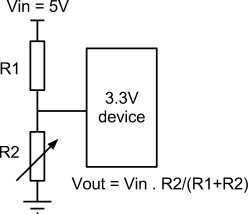
\includegraphics[width=5.5cm]{pictures/voltagedivider}
\label{fig:voltagedivider}
}
\subfigure[Simple 5V to 3.3V communication]{
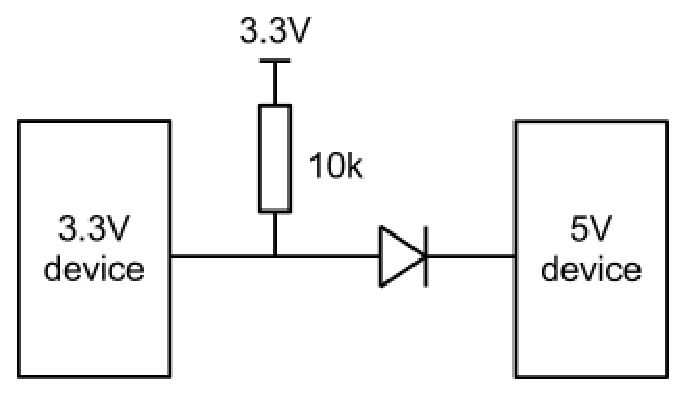
\includegraphics[width=7cm]{pictures/pullupdiode}
\label{fig:pullupdiode}
}
\end{figure}

%\begin{figure}[h!]
%\centering
%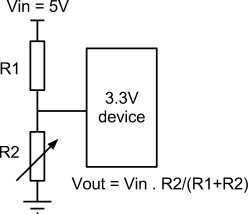
\includegraphics[width=6cm]{pictures/voltagedivider}
%\caption{Voltage divider}
%\label{fig:voltagedivider}
%\end{figure}

%\begin{figure}[h!]
%\centering
%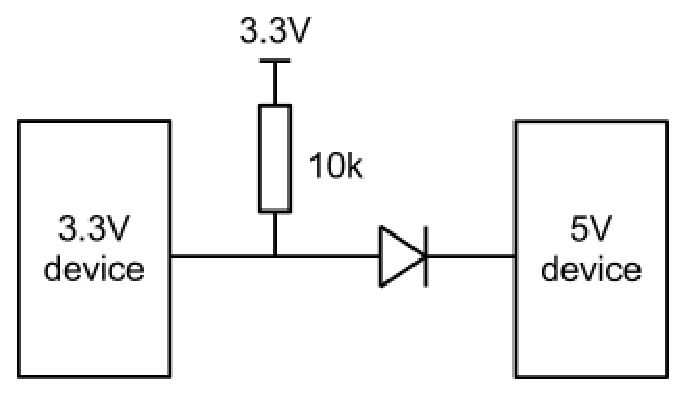
\includegraphics[width=7cm]{pictures/pullupdiode}
%\caption{Simple 5V to 3.3V communication}
%\label{fig:pullupdiode}
%\end{figure}

\section{General Purpose Input Output communication}

A GPIO is a digital hardware pin which can be controlled through the software. It can be used as an input or an output, and since it is digital, it uses the logic levels 0 and 1. Because chips have a limited number of pins (here, 66 on the headers), it sometimes happens that the pin to use necessitates a different MUX setting than the default \verb!MODE0!. The AM3359 has up to 8 different MUX modes per pin, and selecting one of them is going to route the pin to the desired internal logics of the chip. Some pins have no mux modes, such as the A/D pins.
\\
\\
A major evolution of the BeagleBone compared to the BeagleBoard, is that the GPIO pins are directly controllable through software, and that a virtual filesystem can be used to interact with them. Also, one can freely reconfigure the MUX pins. This means that it is not necessary to recompile the kernel when  a MUX value is changed! Then, the usual parameters are the enabling of the GPIO pin, its direction (in/out) and its value to read or write.
\\
\\
The MUX value of a pin is changed under \verb!/sys/kernel/debug/omap_mux!
\\
The rest of the GPIO control is under \verb!/sys/class/gpio/gpioX/!
\\
\\
Below is an example of using a GPIO pin in shell script, a command-line user interface interpreted language. Let us suppose that, for practical reasons, we want to use the first pin available on the P9 header. By looking at the datasheet, we can tell its name is \verb!UART4_RXD!. This means that if we intend to use this pin as a GPIO pin, the MUX has to be set first (mode 7), to configure the pin as \verb!gpio0[30]!. In order to change the MUX setting, we need to retrieve the actual name of the pin as far as the kernel is concerned. The \verb!MODE0! of our pin is named \verb!gpmc_wait0!, so we need to find a file with this name in the \verb!omap_mux! folder.
\\
\begin{lstlisting}[language=sh, basicstyle=\scriptsize]
#/bin/sh

echo 30 > /sys/class/gpio/export                #export the pin, it is now usable
echo 7 > /sys/kernel.debug/omap_mux/gpmc_wait0  #change the MUX setting to 7 (gpio mode)
echo out > /sys/class/gpio/gpio30/direction     #change the direction of the pin
echo 1 > /sys/class/gpio/gpio30/value           #write logical "1" to the pin!
echo 30 > /sys/class/gpio/unexport              #unexport the pin for a clean exit
\end{lstlisting}

Note that this method is the simplest, but also the slowest. If the speed at which the toggle can occur, and its preciseness in time are higher, two options are available:
\begin{itemize}
\item Direct register access: by mapping into memory the registers (as described in the PWM chapter), the actual delays of context switching from userspace to kernel space is bypassed, but there is an extensive documentation work to make to find register addresses (see AM335x technical reference manual \cite{amtrm})
\item PRU: the Programmable Real-time Unit is a dedicated unit capable of real-time in the AM3359 chip. It is a very complicated and time intensive solution, but it yields the best results.
\end{itemize}

Some interesting features of the GPIO pins is that, depending on their setting, they can be used to generate PWM output, for TTL communication such as I$^{2}$C or SPI and UARTs, or to set timers and interrupts.

\section{Communication protocols}

A UART is an asynchronous configurable hardware device usually used for serial communcation. Its goal is to translate bytes into series of bits and inversely, to minimize the number of wires used. It is associated with a protocol, such as RS-232.
\\
\\
SPI is a synchronous serial data link, developed by Motorola. It is based on a master/slave architecture, in full duplex mode. It uses 4 wires: a serial clock, a master output (resp. slave input) and a master input (resp. slave output), and a slave select.
\\
\\
I$^{2}$C is a serial bus, developed by Philips. It uses a multi-master/slave architecture, with 2 wires only: a serial clock and a data line. 
SPI has a higher throughput than I$^{2}$C, and consumes less power since it does not use pull-up resistors. On the other hand, I$^{2}$C uses fewer lines, is easier to debug and is more adapted to multinode communciation. A lot of electronic module boards embedding dedicated chips typically use SPI/I$^{2}$C.
\\
\\
Note that a level-shifter (3.3/5\,V) is usually necessary for I$^{2}$C, since the data line is bidirectional. With SPI, it is possible to implement electronics to avoid using a level-shifter, but it is recommended nonetheless.

\chapter{Realisations}

This chapter contains the realisations and for each thema there are a number of programs that depicts the functionnalities of the subject in question. The correspondance between thema and program was given in table~\ref{tab:1}.

\section{Sensors: using the A/D conversion}

The following sensors have been integrated:
\begin{itemize}
\item Light Dependant Resistor (LDR)
\item Negative Temperature Coefficient (NTC) thermistor
\item 3-way accelerometer
\item IR distance sensor
\end{itemize}

The complexity of integrating such sensors is highly variable. For instance, a distance sensor has a basic linear output, therefore a simple multiplication will give the actual distance seen by the integrated sensor. This linear behaviour is inherently linked to the complexity of the sensor (it costs around 10 euros). On the other hand, the thermistor used here is a very simple sensor and consists of a material which resistance varies non-linearly with the temperature. This implies that the complexity is going to be found on the side of the receiving board: the voltage received has to be converted to a resistance, and then this resistance value will allow the calculation of the actual temperature.
\\
\\
The law in question is called Steinhart and Hart's law, 

\begin{math}
1/T= A + B \cdot ln(R/Rt) + C \cdot ln(R/Rt)^{2} + D \cdot ln(R/Rt)^{3}
\end{math}
\\
\\
The coeffecients A to D are given in the datasheet. Note that here, for some reason, 
the first 2 coefficients given in the datasheet (A1, B1) take the exponent specified in the head of the table whereas C1 and D1 take the unchanged coefficients as given in the cell.

\begin{figure}[h!]
\centering
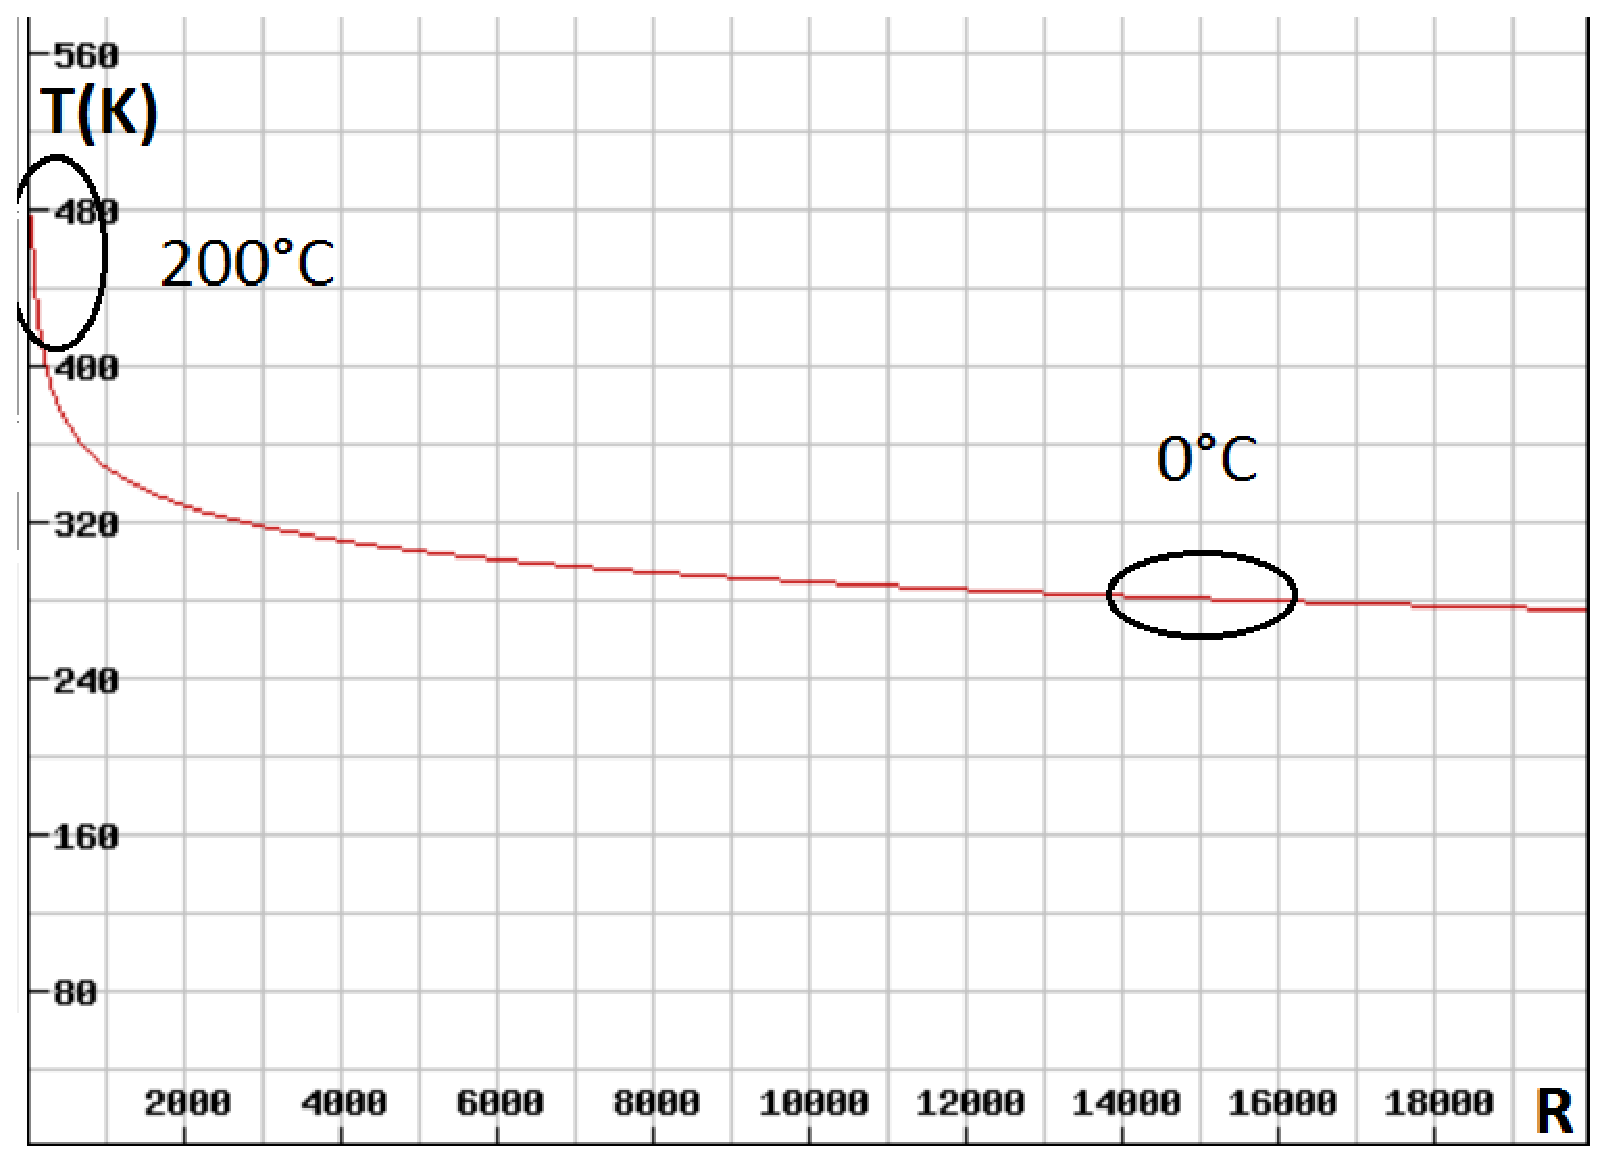
\includegraphics[width=7cm]{pictures/ntcthermistor}
\caption{R=f(T) for this NTC thermistor}
\label{fig:ntcthermistor}
\end{figure}

Figuring out the equation and plotting it is purely essential: if it so happened that the resistor of the voltage divider was ill-calibrated (Vmax=1.8\,V), the board would surely get damaged.
The precision given in the datasheet of the thermistor is 0.005�C in the [25;125�\,C] interval, but since the voltage fed to the thermistor is not 5\,V and that R1 in the voltage divider is not precisely 20k$\Omega$ (resistances are usually given with a $\pm$ 5\% precision), and that the thermistor has to be calibrated, the final precision is lowered considerably! But, using appropriate tools such as a digital voltmeter, it is possible to precisely measure R1, V$_{in}$ and calibrate the thermistor to achieve a <1\% error.
\\
\\
The LDR results are barely exploitable, since the details to building the logartithmic curve are not given and the graph provided is of too poor quality for actual readings. To give an idea what a lux actually represents, consider the approximations given in table~\ref{tab:1}.

\begin{table*}
\centering
\begin{tabular}{|c|c|c|c|} \hline
\textbf{Lux}   & \textbf{Context} \\
\hline
0.001   & Night\\
\hline
0.1   & Emergency lightnings\\
\hline
50   & Poorly lit room\\
\hline
100   & Very cloudy day\\
\hline
1000  & Well lit room\\ 
\hline
10000  & Daylight\\ 
\hline
100000  & Direct sunlight\\ 
\hline
\end{tabular}
\caption{Light in Lux in various situations}
\label{tab:1}
\end{table*}

\section{Communication: in and out}

On the cape built for purposes of demonstration, one can find 2 push buttons and an HD44780 LCD controller display. Both of these elements use the GPIO, one as an input and the other as an output.
The HD44780 controller is a chip that makes it easy to communicate with an alphanumeric LCD display. Though these kits can easily being turned into serial peripherals, they originally are parallel devices that either operate in 4 or 8 bits mode for the data and 3 bits for the control. The actual minimum of GPIO pins to drive such a display kit is 6, because it is usually not useful to read from the device, and therefore one pin (R/W) can be directly shortened to ground if unneeded.
\\
\\
The \verb!demo_lcd! program makes use of the \verb!lcd! library that depends itself from the \verb!gpio! library. The gpio library provides a set of C functions to initialize a pin, write to it, read from it. The lcd library includes the initialization of the screen, the timings and basic commands of the HD44780 controller. The protocol for the HD44780 as well as the usual wiring are recapitulated on figure figure~\ref{fig:pinoutHD44780} and table[XX]. Because the screen has been used on a transversal copper-plated PCB, the screen pins pan along pins not natively configured as gpio pins, thus the mux must be preconfigured for some pins (which default mode is a dedicated function) and not for some others (which default mode is a usable GPIO configuration).
\\
\\
Because the files used to read/write from/to the gpio are not usual files, the classic \verb!libc fprintf(3)! function is not guaranteed to work in an unbuffered manner. This can be solved by closing the file each time it has been written to. The \verb!libc! function \verb!fflush(stdout)! can be used instead, but is probably not defined for special files either. The system calls \verb!open(2)! and \verb!write(2)! should solve the problem

\begin{figure}[h!]
\centering
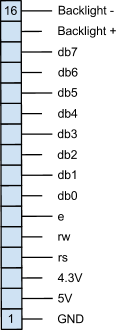
\includegraphics[width=2cm]{pictures/pinoutHD44780}
\caption{Pinout for a usual HD44780 controller}
\label{fig:pinoutHD44780}
\end{figure}


\section{Pulse-Width Modulation}

The Pulse-Width Modulation is a technique in which short bursts of energy of variable length are fed to an electrical device at a rate sufficient for the load to see a uniform wave, thus allowing any type of wave (sine, constant ...),  to be approximated from a square wave with a fixed amplitude. Historically, it appeared to prevent the wasting of energy in resistors when the electric load was in 'idle' mode.
\\
\\
PWM is traditionally used to control servomotors (1\,kHz), blinking LEDs at very precise frequencies (40\,kHz: carriers in the infrared terminology) or in audio amplifiers (100\,000\,Hz), but is now also used in fan control on recent motherboards (25\,kHz), in electric heating systems or stoves (<1\,Hz) and even in lamp dimmers (120\,Hz).
\\
The main characteristics are the switching frequency and the duty cycle. Whilst the former controls the form of the desired output wave as seen from the electrical load, the latter controls its actual amplitude by averaging it at a higher frequency.
\\
Here we use a buzzer to demonstrate two ways of playing a melody:
\begin{itemize}
\item with PWM emulation (GPIO)
\item with real PWM
\end{itemize}

At the time this project was started, there was no support for PWM in the applied Linux kernel. Therefore, a GPIO bitbanging solution was implemented. It relies heavily on the \verb!nanosleep()! function. But of course, since we do not work in real-time, this method has terrible results! Because the output is a music played on a buzzer, it is not necessary to use an oscilloscope to detect that the result is floppy, as notes are out of tune. Nonetheless, the musical theme is easily recognized. A way to slightly improve this method is to use soft real-time scheduling privileges, by using the \verb!sched_setscheduler(2)! system call with the \verb!SCHED_FIFO! policy.
\\
\\
However, with the newest kernel version (3.2.0+) it became possible to implement a real PWM control for the buzzer. The gpio.txt file, part of the kernel documentation, explains how it has to be set up. Because system clocks are disabled by default, the one relevant to the PWM output to use has to be enabled. But since this special register is not yet mapped in memory, the system call \verb!mmap(2)! has to be used on the portion of \verb!/dev/mem! which contains the system clocks registers. Also, by referring to the SRM of the BeagleBone, we can see that the PWM pin we intend to use necessitates that the MUX mode be set to 6. Once this is configured, the files in the virtual filesystem found under \verb!/sys/class/pwm/ehrpwm.X:Y/! can be used, namely \verb!period_freq(frequency in Hz)!, \verb!duty_percent! (0-100\%) and \verb!run! (0/1).

\section{Timers / Interrupts}

Though microcontrollers usually make an extensive use of timers, they're not actually used all that much on embedded Linux. Depending on the use and the precision needed, timestamps which count time from an arbitrary point in time are an acceptable solution. A real-time operating system probably provides better interfaces with timers.
\\
\\
The timer pins from the GPIO can be a bit misleading, they actually are used to drive synchronous peripherals with an internal circuit. For instance, one could get rid of the quartz that drives a PIC microcontroller and connect the clock pins of the PIC directly to that of the BeagleBone.
\\
\\
External interrupts are usable through the \verb!poll(2)! system call, which when specified a file descriptor will hang until an interrupt has been triggered. The path to specify here is that of the value file of the GPIO.
The conditions under which an interrupt should be triggered are configurable in the gpio sysfs interface, namely in the \verb!edge! file. The options are \verb!none!, \verb!rising! (set trigger from low to high), \verb!falling! (set trigger from high to low) and \verb!both!, and the default is \verb!none!.
\\
\\
The IR programs developed for this project demonstrate two possible ways to read an IR signal from basically any remote controller, record it and compare it to a list of signals:
\begin{itemize}
\item file polling with delays
\item the use of GPIO interrupts (compare CPU usage, precision)
\end{itemize}

While both methods have proven to work to read, record and compare an IR signal, the precisions are an order of magnitude below. The worst case result of the first solutions was 6:8 which is an maximal error of 25\%. Nonetheless, with this solution the results usually have an error of less than 10\% which is sufficient for reading and comparing, although it would certainly be impossible to write the message back through another circuit.
\\
\\
The second method uses interrupts and timestamps. If we base our reasoning on the hypothesys (inevitably wrong, but still) that the interrupts have about the same latency, then the max error is 0, or that of the timestamp. Here, we use the \verb!gettimeofday(2)!, which precision is the order of a microsecond. Since the IR switching frequencies are more in the milliseconds, our worst case has 10 times the resolution needed. In reality, the error induced by the interrupt handling is a little less than 2\% and the precision is 100 times better.

Functions for timers:
\verb!<time.h> <signals.h>!
\verb!timer_create(2)!
\verb!timer_settime(2)!
\verb!timer_gettime(2)!

\verb!setitimer(2)!
\verb!getitimer(2)!

\verb!<sys/timerfd.h>!
\verb!timefd_create(2)!
\verb!timerfd_settime(2)!
\verb!timerfd_gettime(2)!

\section{Video feed over http}

Because the camera used for this project is a UVC (USB Video Device Class) camera, it worked straight out of the box with the image and \verb!mjpeg-streamer!. This package is able to grab JPEG pictures directly from the camera and stream them to a webserver. But because several instances of mjpeg-streamer can run, it is possible to grab a picture, save it and execute a script from one instance, and stream the modified pictures with a second instance.
\\
\begin{lstlisting}[language=bash, basicstyle=\scriptsize]
run.sh:
./mjpg_streamer -i "./input_uvc.so -d /dev/video0" 
		-o "./output_file.so -f /tmp/pics/raw/ -d 15000 -c ./bla.sh" &
./mjpg_streamer -i "./input_file.so -f /tmp/pics -r"
		-o "./output_http.so -w www" &
\end{lstlisting}

To demonstrate a basic overlay, ImageMagick's convert function is used on the input jpeg, and the output jpeg is sent to the stream folder. Here we use a double overlay to make sure the text is visible on any colour. The problem here is that the creation of the overlay requires that the input jpeg be uncompressed, modified and recompressed, thus limiting the framerate to less than 2 fps with up to 10\% CPU consumption. By increasing the \verb!nice! value, it is possible to achieve 50\% more performance, with a CPU usage of 15\%.
\\
\\
\begin{lstlisting}[language=sh, basicstyle=\scriptsize]
convert.sh:

#!/bin/sh
dir="/tmp/pics/raw/"

temp_k=`/home/root/code/thermistor`
temp= echo "\$temp_k - 273.15" | bc
nice -n -20 convert \$1 -gravity south \
-font /usr/share/fonts/ttf/LiberationMono-Bold.ttf \
-stroke '#000C' -strokewidth 2 -annotate 0 'Temperature : '\$temp \
-stroke none -fill white     -annotate 0 'Temperature : '\$temp \
/tmp/pics/test.jpg !
rm \$dir*.jpg
\end{lstlisting}

If we want to build a system that take pictures, applies an overlay onto them and streams them back to monitor something, then the system should be able to reboot by itself in case it crashes. Therefore, we need to add entries to the init.d rules, with the daemon update-rc.d

\section{Database and CGI scripts}

It could be useful in the case of a production application to easily monitor the application from a remote location. In conjunction to a real webserver with PHP modules, a SQL relational database can be set up to store data. Programs in C (or for that matter, any language) can use a specific API to write to this database. A page in PHP can then integrate these values directly into the page sent to the user (in html after the conversion). It is also possible to control the system from the web, by using CGI (Common Gateway Interface) scripts. It is to note that these scripts can also be written in many languages, the most common ones being C and perl.
\\
\\
Here, SQLite is used as an alternative to the classic MySQL for small databases. It is lightweight and its structure is much simpler. \verb!lightttpd! is a server with equivalent characteristics.
Both packages can be intalled from \verb!opkg!: \verb!lightttpd! and \verb!sqlite3!.
It is possible to create the database from the API, but it is something usually done from the command line interface. The basic commands are presented below:
\\
\\
\begin{lstlisting}[language=bash, basicstyle=\scriptsize]
sqlite3 test.db						# create and open test.db
> CREATE TABLE test (id integer primary key, value text); # create a table inside the db
> INSERT INTO "test" VALUES(1,'900;500;1400');		# insert a row
\end{lstlisting}

Another interesting possibility of webservers is the execution of CGI script, on the target. This allows a remote user to execute code on the server and possibly get a return value. It is possible to pass arguments to the CGI script using the \verb!POST/GET! methods. The CGI can be written in any language, but here we use perl to show the simplest example.

The webserver chosen here is lighttpd, but Cherokee would have been an equally valid choice when it comes to lightweight, stripped-down, fast servers for embedded systems.

It was installed using
\\
\\
	\verb!opkg install lighttpd lighttpd_mod_cgi!
\\
\\
To enable CGI scripts, simply edit \verb!/etc/lighttpd.conf!, and uncomment the 3 lines concerning CGI (\verb!mod_cgi! in \verb!server.modules!, and the CGI portion containing \verb!cgi.assign!)
lighttpd creates a default \verb!index.html! file in \verb!/www!, where the server points. This file was modified to include buttons that turns a led on or off, using the \verb!led.cgi! script, written in perl. When the user clicks a button, it submits a form using the POST method to call a CGI script. The script can receive arguments and usually has to give HTML code back, thus implying the page changes. A way to circumvent this problem is to use the AJAX technologies.
\\
\\
Though this was not implemented here, a central element to CGIs and databases is the PHP language. To put it in a nutshell, PHP allows the dynamic generation of webpages depending on the SQL database. Another very powerful technology to combine here is Javascript and the jQuery library to dynamically modify code inside a page from the client-side, and beneficiate from the callback of jQuery when invoking a script.
Note on embedded systems: if maintaining a connection to the server is primordial, the options besides using long polling are very limited.


\chapter{Conclusion: Linux on ARM vs other RISC architectures }

It is quite clear that beyond the similarities of the architecture (PWM, timers, interrupts), microcontrollers (PIC, AVR) and microprocessors (typically ARM) serve a different purpose. A microcontroller, though some can embed an tiny C OS, is a very simple machine, whereas ARMs are much more complex and can run a real OS, namely the Linux kernel.
\\
\\
The range of use of an ARM easily covers that of the microcontroller and extends it with powerful features such as the use of a camera. But doing the simplest of things such as blinking a LED at a very precise frequency can easily become an impossible to fulfill task in the user-space, and requires coding in the kernel. Developing in the kernel is a much tougher challenge and requires very advanced knowledge of the environment. A wild pointer would likely crash the system, and the try/fail/try/succeed approach would be very time consuming.
Therefore, appropriate considerations need to be taken into account when choosing the architecture of a system. What can be done on a microcontroller should probably be done on a microcontroller (an IR system, basic use of sensors, servos), and what requires a more powerful system (webserver with database, logins, file operations, cameras ...) should lead to using an ARM (in conjunction to a DSP for audio/video usually). It sums up to this rule of thumb:
\textit{``There are hardware mistakes that no amount of software can patch''}.
\\
\\
In my opinion, the best approach to a complex system consisting partly of real-time software is an hybrid ARM/PIC, with an I$^{2}$C bus for the communication. The distinction between the (possible) user-interface and the real-time part of the system would be made clear, and the only drawback I can really think of is that the real-time part would receive orders with a slight delay.
Another, more Real-Time specific approach would be to use the PRU (Programmable Real-Time Unit) from the AM3359, but it is inevitably much more work than the hybrid solution.



%%%%%%%%%%%%%%%%%%%%%%%%%%%%%%%%%%%%%%%%%%%%%%%%%%%%%
% Der Anhang (andere Sektionsnummerierung)
%%%%%%%%%%%%%%%%%%%%%%%%%%%%%%%%%%%%%%%%%%%%%%%%%%%%%
%%\appendix
% Hier werden die Anhänge eingebunden
% TODO : weitere Kapitel in my_appendices.tex eintragen
%%% Hier die Kapitel des Anhangs einf�gen
%% Anhang
%

\chapter{Hintergrundwissen zur Grafikeinbindung}

Ganz viele Dinge, die nicht so wichtig sind, wenn man sich mit dem Thema schon
auskennt.


\footnotesize{
\begin{thebibliography}{50}
\bibitem {bbgts} BeagleBone getting started guide: \url{http://beagleboard.org/static/beaglebone/a3/README.htm}
\bibitem {bbsrm} BeagleBone SRM Datasheet:\url{http://beagleboard.org/static/beaglebone/a3/Docs/Hardware/BONE\_SRM.pdf}
\bibitem{kgpio} Kernel documentation gpio.txt: \url{http://www.kernel.org/doc/Documentation/gpio.txt}
\bibitem {agimg} Angstr�m project, official demo image: \url{http://www.angstrom-distribution.org/demo/beaglebone/}
\bibitem {amtrm} Texas Instruments, AM3359 TRM Datasheet: \url{http://www.ti.com/product/am3359}
\bibitem {putty} Putty project homepage: \url{http://www.chiark.greenend.org.uk/~sgtatham/putty/download.html}
\end{thebibliography}}


% evtl. Abkuerzungsverzeichnis (z.B. Paket nomenclature)

%%\printindex                     % Wenn ein Index erstellt werden soll, muss
                                %  diese Zeile aktiviert werden
                                %  Zusaetzlich oben das Paket einbinden und \makeindex

\end{document}



